\section{敏感性与可行性检验}

图~\ref{fig:sens}给出第一问对返航安全余量的离散敏感性。10\%到20\%时最少架次和能耗不变，说明该范围内最优组批具备余量；30\%发生组批跳变，最少架次增为20；40\%则因S004的14~kg整箱水而出现不可行。这里的不可行是规定“单点直接往返”和“货箱不可拆”共同作用的结果，不能通过在第一问中增加架次消除。

\begin{figure}[H]\centering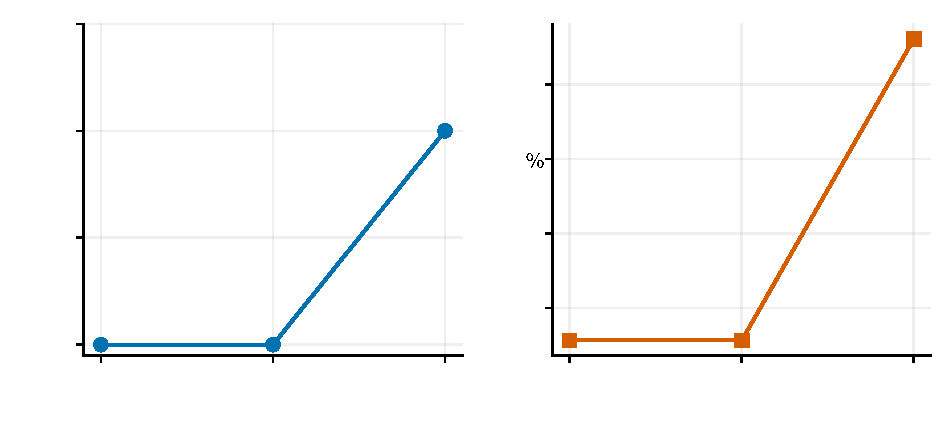
\includegraphics[width=.9\textwidth]{../figures/sensitivity.pdf}\caption{可行区间内安全余量对最少架次和能耗的影响}\label{fig:sens}\end{figure}

跨问回代检查逐箱唯一性、载荷和体积、各航段能耗、返航SOC、医疗及首批硬时限、同机与同电池任务区间、充电区间、中继任务与组件区间以及通信连续性。问题二最紧硬时限松弛257.26~s；问题三为112.86~s。两问均无硬时限违规，最低运输SOC比20\%下限高0.1676个百分点。问题三最小中继SOC为23.6510\%，最小链路预算裕量仅0.0061~dB。该极小通信裕量不能解释为抗扰动稳健；一旦链路附加损耗上升，应重选悬停点或修改航线和起飞时刻。

通信核验的区间下界采用DEM全像元最高地形与视线高度保守比较，且把运动端点到固定端点的整个扫掠区域纳入，因此已证实的区间不依赖于离散采样间隔。由于题目只给出静态DEM和固定衰落裕量，暴雨、瞬时干扰、阵风、地物变化以及GNSS误差仍位于模型适用范围之外。
